
\chapter{Biased Random Key Genetic Algorithm}

\section{Algoritmos Genéticos}

Los \textit{Genetic Algorithms} (GA) \cite{Goldberg} están motivados en el concepto de supervivencia del más apto para encontrar soluciones óptimas o casi óptimas a los problemas de optimización combinatoria. Los GA hacen una analogía entre una solución y un individuo que pertenece a una población, donde cada individuo es un cromosoma que codifica una solución. Un cromosoma consiste en una cadena de genes. Cada gen, llamado alelo, toma un valor de algún alfabeto. Cada cromosoma tienen asociado un nivel de condición física que está correlacionado con el correspondiente valor de la función objetivo de la solución que codifica. 

\bigskip

Los algoritmos genéticos manejan un conjunto de individuos que forman una población a lo largo de varias generaciones. En cada generación se crea una nueva población con individuos provenientes de tres fuentes distintas. La primer fuente de individuos es el conjunto de soluciones elite, es decir los individuos de mejor condición física. La segunda fuente de individuos son los individuos resultantes del \textit{crossover}. El \textit{crossover} es el método por el cual se obtiene un nuevo individuo a partir de otros dos individuos. Por último se completa la nueva generación con individuos mutantes. Los mutantes son individuos generados al azar con el fin de escapar de atrapamientos en mínimos locales y diversificar la población. 

\bigskip

El concepto de supervivencia del más apto puede aparecer en los algoritmos genéticos de varias formas, dependiendo de la implementación en particular. Generalmente las soluciones de mayor aptitud física pasan directamente a la nueva generación. Además en el método del \textit{crossover}, cuando los individuos son seleccionados para aparearse y producir descendencia, aquellos con mejor aptitud física tienen mayor probabilidad de ser elegidos para generar descendientes y mayor probabilidad de transmitir sus genes a sus hijos.

\section{Random Key Genetic Algorithm}

Los \textit{Random Key Genetic Algorithm} (RKGA) fueron introducido por Bean \cite{Bean}. En los RKGA, los cromosomas o individuos son representados por un vector de números reales generados al azar en el intervalo [0, 1]. El decodificador es el responsable de convertir un cromosoma en una solución del problema de optimización combinatoria, para el cual se calcula su valor objetivo o aptitud física. Los RKGA evolucionan una población de vectores de números reales aleatorios sobre una serie de iteraciones llamadas generaciones. La población inicial se compone de $p_t$ vectores de claves aleatorias. Todos los vectores contienen la misma cantidad de claves aleatorias llamadas alelos. Cada alelo se genera independientemente al azar en el intervalo real [0, 1]. Después de obtener las soluciones utilizando el decodificador, se calcula la aptitud de cada individuo de la población, luego la población se divide en dos grupos de individuos. Se obtiene por un lado un pequeño grupo de individuos de élite. Estos son los individuos con los mejores valores de aptitud física. Denotamos el tamaño del conjunto de elite como $p_e$. Por el otro lado se conforma el grupo de todos los individuos restantes llamado el grupo de no-elite y su tamaño es $p_t-p_e$. Todo individuo del conjunto de elite tiene mayor aptitud física que cualquier individuo del conjunto de no-elite y el tamaño del conjunto de elite es menor al tamaño del conjunto de no-elite, es decir $p_e<p_t-p_e$. Con el fin de evolucionar a la población, un RKGA utiliza una estrategia elitista ya que todos los individuos de élite de la generación $k$ se copian sin cambios a la generación $k+1$. Esta estrategia mantiene un seguimiento de las buenas soluciones encontradas durante las iteraciones del algoritmo que resulta en una heurística de mejora monotónica. En el RKGA los individuos mutantes se generan a partir de vectores de números reales aleatorios, de la misma manera que los individuos de la población inicial. Con la población $p_e$ (elites) y la población $p_m$ (mutantes), un conjunto adicional de tamaño $p_t - p_e - p_m$ es requerido para completar la generación $k+1$. Los individuos que completan la nueva generación se obtienen mediante el proceso de \textit{crossover}, donde los padres son elegidos al azar sobre toda la población y cada padre tiene la misma probabilidad de transmitir sus genes al individuo resultante.

\section{Biased Random Key Genetic Algorithm}\label{sec:brkga}

El \textit{Biased Random Key Genetic Algorithm} (BRKGA), difiere del RKGA en la forma en que los padres son seleccionados para el \textit{crossover}. En el BRKGA, cada elemento se genera combinando un elemento seleccionado al azar del conjunto de elite y el otro de la partición no-elite. En algunos casos el segundo padre se selecciona de toda la población mientras sean dos padres diferentes. Se permite la repetición en la selección de un padre, entonces un individuo puede producir más de un hijo. En la figura \ref{fig:evolucion} se puede observar como funciona la evolución. Como el tamaño del conjunto de elite es menor al tamaño del conjunto de no-elite ($p_e < p_t - p_e$), la probabilidad de que un individuo de elite sea seleccionado para el apareamiento es mayor que la de un individuo no-elite. Por lo tanto un individuo de elite tiene una mayor probabilidad de transmitir sus genes a las generaciones futuras. Otro factor que contribuye a este fin es el \textit{parameterized uniform crossover} (Spears y DeJong \cite{SpearsDeJong}), el mecanismo utilizado para implementar el apareamiento en BRKGA. Sea $\rho_e > 0,5$ la probabilidad de que un descendiente herede el alelo de su padre de elite, sea $n$ el número de alelos de un individuo, para $i =1,...,n$ el i-ésimo alelo $c_i$ del descendiente $c$, este alelo $c_i$ toma el valor del i-ésimo alelo $e_i$ del padre de elite $e$ con una probabilidad $\rho_e$ y el valor del $e'_i$ del padre no-elite con probabilidad $1-\rho_e$. Como $\rho_e > 0,5$, entones $\rho_e > 1 - \rho_e$, por lo tanto es más probable que el individuo resultante herede características del padre de élite que las del padre de no-élite. Si el decodificador se implementa de forma tal que cualquier vector de números reales se convierta en una solución válida, entonces el cromosoma resultante del \textit{crossover} siempre decodifica en una solución válida del problema de optimización combinatoria.

\bigskip

En la figura \ref{fig:biasCrossover} se puede observar como funciona el \textit{parameterized uniform crossover}. El primer vector de alelos es de un individuo de elite, el segundo vector de alelos es de un individuo no-elite. Se decide que alelos tomará el individuo resultante utilizando un vector de números reales aleatorios del mismo tamaño que los vectores de alelos. Los números reales aleatorios toman un valor real en el intervalo [0,1]. En este ejemplo se utiliza un $\rho_e = 0.70$ incrementando la probabilidad de que el cromosoma resultante obtenga los alelos del cromosoma elite.

\begin{figure}[h]
	\caption{Bias Crossover}
	\centering
	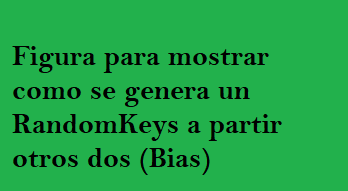
\includegraphics[width=15cm]{BiasCrossover}
	\label{fig:biasCrossover}
	\floatfoot{En la figura \ref{fig:biasCrossover} podemos observar como el individuo resultante hereda el primer alelo del individuo de no-elite por que el número real aleatorio en la primera posición resulto mayor a $0.70$}
\end{figure}

\begin{figure}[h]
	\caption{Evolución de una Población}
	\centering
	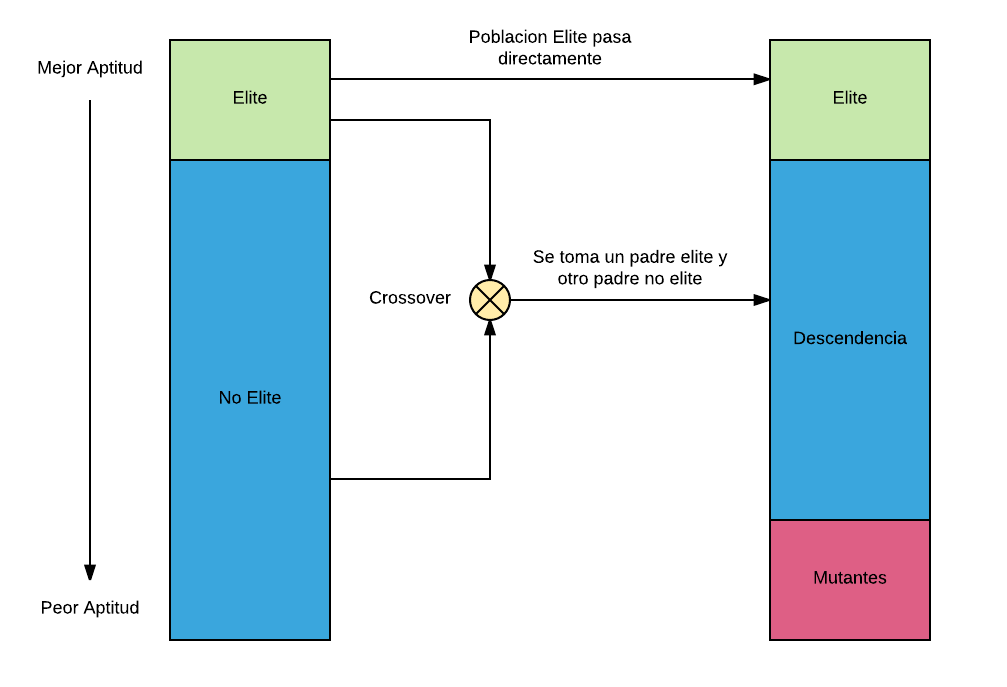
\includegraphics[width=16cm]{EvolucionPoblacion}
	\floatfoot{En la figura \ref{fig:evolucion} los individuos son ordenados por su aptitud y marcados como elite y no-elite. Vemos como los individuos de elite pasan directamente a la siguiente generación. Un porcentaje pequeño de la nueva generación es conformado por individuos mutantes, generados al azar como la población inicial. Y complementa la nueva población los individuos generados por el proceso de \textit{crossover} entre un individuo elite con un individuo no-elite.}
	\label{fig:evolucion}
\end{figure}

\section{Decodificador del BRKGA}

Una característica importante para mencionar del BRKGA es que el decodificador es el único modulo del algoritmo que requiere conocimiento del dominio del problema. El decodificador transforma un vector de números reales aleatorios en una solución válida del problema. El decodificador funciona como un adaptador, por lo tanto si hacemos un decodificador para otro problema podríamos reutilizar el modulo del BRKGA.

\bigskip

En el caso de mi implementación del BRKGA, entre cada generación se ejecuta una búsqueda local sobre las mejores soluciones de la población. Como estas búsquedas locales trabajan con una solución decodificada, luego de optimizar una solución se debe actualizar su vector de números reales. Es por eso que implementé un algoritmo capaz de convertir una solución $s$ del problema en un vector $v$ de números reales aleatorios tal que al decodificar el vector $v$ se obtenga la solución $s$ inicial. De este modo, una vez que se mejora una solución, se actualiza su vector de números reales aleatorios que lo representa y luego el BRKGA sigue su curso normal. 

